\documentclass[aps,prd,twocolumn,showpacs,superscriptaddress,nofootinbib]{revtex4-2}

\usepackage{amsmath,amssymb}
\usepackage{graphicx}
\usepackage{booktabs}
\usepackage{siunitx}
\usepackage{hyperref}

% Canonical counts pipeline (Phase 5v: freshness gate).
% Auto-generated by update_counts.py — 2026-04-24T19:44:03.140400
% Do not edit manually. Run: uv run python scripts/update_counts.py
\newcommand{\totaltheorems}{3993}
\newcommand{\substantivetheorems}{3882}
\newcommand{\placeholdertheorems}{111}
\newcommand{\axiomcount}{1}
\newcommand{\sorrycount}{0}
\newcommand{\sorrypercent}{0.0}
\newcommand{\leanmodules}{167}
\newcommand{\leandefinitions}{3297}
\newcommand{\pythonmodules}{68}
\newcommand{\testfiles}{59}
\newcommand{\totaltests}{2836}
\newcommand{\figurecount}{111}
\newcommand{\notebookcount}{54}
\newcommand{\papercount}{19}
\newcommand{\aristotleproved}{322}
\newcommand{\aristotleruns}{44}
% --- Paper 18 / Phase 5t per-section counts (FermiHubbardDimer.lean) ---
\newcommand{\fhdTotal}{143}
\newcommand{\fhdWaveTwo}{13}
\newcommand{\fhdWaveThree}{6}
\newcommand{\fhdWaveFour}{22}
\newcommand{\fhdWaveFive}{22}
\newcommand{\fhdWaveSixABC}{38}
\newcommand{\fhdWaveSixExtra}{15}
\newcommand{\fhdWaveSeven}{19}
\newcommand{\fhdWaveEight}{8}


\newcommand{\GN}{G_{N}}
\newcommand{\GNobs}{G_{N}^{\rm obs}}
\newcommand{\GNemerg}{G_{N}^{\rm emerg}}
\newcommand{\GNsak}{G_{N}^{\rm Sak}}
\newcommand{\Lambdauv}{\Lambda_{\rm UV}}
\newcommand{\Mpl}{M_{P}}
\newcommand{\Nf}{N_{f}}
\newcommand{\aADW}{\alpha_{\rm ADW}}
\newcommand{\Gc}{G_{c}}

\begin{document}

\title{Linearized Einstein Equations from Anderson--Higgs Tetrad Condensation:\\
A Lean-formalized treatment with the Sakharov--Adler closed form
and a tracked-hypothesis $\aADW$}

\author{John G.\ Roehm}
\affiliation{NetRxn Foundation}

\date{\today}

\begin{abstract}
We formalize the linearized Einstein field equations in the Anderson--Higgs
tetrad condensation (Akama--Diakonov--Wetterich, ADW) framework as the
load-bearing first wave of Phase 6a of the SK--EFT Hawking project. Working
in the broken-symmetry phase of the ADW four-fermion theory at coupling
$G > \Gc$ on a flat Minkowski background, we (i) prove the linearized
Einstein tensor in momentum-space de Donder gauge,
$G^{(1)}_{\mu\nu}(k) = -\tfrac{1}{2}\,k^{2}\,\bar{h}_{\mu\nu}$, with full
Lean-verified algebra of trace-reversal and the spin-2 kinetic operator;
(ii) record the Sakharov--Adler closed form for the induced Newton constant,
$\GNsak = 12\pi/(\Nf\,\Lambdauv^{2})$, and tie it to the existing ADW
critical-coupling theorem $\Gc = 8\pi^{2}/(\Nf\,\Lambdauv^{2})$ via the
exact algebraic identity $\GNsak = (3/2\pi)\,\Gc$; (iii) define the
ADW emergent Newton constant
$\GNemerg(\Lambdauv,\Nf,\aADW) = \aADW \cdot \GNsak$ with the
ADW microscopic coefficient $\aADW$ as a tracked-hypothesis
dimensionless parameter; (iv) establish the correctness-push biconditional
that $\GNemerg = \GNobs$ holds iff
$\Lambdauv^{2} = \aADW \cdot 12\pi/(\Nf\,\GNobs)$, which at the natural
Planck anchor $\Lambdauv = \Mpl$ reduces to $\aADW \cdot 12\pi = \Nf$,
consistent with $\aADW \in [0.40,1.27]$ for SM $\Nf \in \{15,16,45,48\}$
and the Vergeles natural range $[0.1,10]$.

A directed deep-research survey of the primary ADW literature
(Diakonov 2011, Vladimirov--Diakonov 2012, Hebecker--Wetterich 2003,
Wetterich 2022, Vergeles 2025, Volovik 2022/2024) finds that no published
work computes $\aADW$ in closed form. The literature does support three
structural Vergeles-derived properties:
\textbf{positivity} ($\aADW > 0$ strictly inside the broken phase, from
Osterwalder--Schrader reflection-positivity \cite{Vergeles2025}),
\textbf{critical-limit collapse} ($\aADW \to 0$ as $G \to \Gc^{+}$,
mean-field linear scaling \cite{VladimirovDiakonov2012}), and
\textbf{deep-gap reduction} to Sakharov--Adler ($\aADW \to 1$ as
$G/\Gc \to \infty$, Adler 1982 normalization \cite{Adler1982}).
We encode these as three Lean Props, prove that the linear
ansatz $\aADW(G/\Gc) = 1 - \Gc/G$ satisfies all three, and deliver
the numerical anchor $\aADW(2\,\Gc) = \tfrac{1}{2}$ giving
$\Mpl^{\rm emerg} \approx 0.7\,\bar{\Mpl}$ at $\Nf=15$.
The full formalization (\texttt{LinearizedEFE.lean},
$35$ theorems) is zero-sorry, introduces zero new axioms, and adds zero
heartbeat overrides. The closed-form value of $\aADW$ awaits the
missing one-loop $\langle h^{a}_{\mu}(p)\,h^{b}_{\nu}(-p)\rangle$
calculation in the broken phase, which we identify as a natural
follow-up paper.
\end{abstract}

\pacs{04.20.-q, 04.50.-h, 04.60.-m, 11.15.-q}

\maketitle

%% ================================================================
\section{Introduction}
\label{sec:intro}

The Akama--Diakonov--Wetterich (ADW) program~\cite{Akama1978,Diakonov2011,
HebeckerWetterich2003,Wetterich2022,VladimirovDiakonov2012} treats the
metric tensor as a composite bilinear of more fundamental Grassmann fields,
emerging via spontaneous symmetry breaking $L_{c} \times L_{s} \to L_{J}$ of
the local-Lorentz frame. In the broken-symmetry phase, the
tetrad $e^{a}_{\mu}$ condenses, six Nambu--Goldstone modes are absorbed by
the spin connection, and two massless graviton helicities propagate
on a flat Minkowski background~\cite{Volovik2022Counting}.

The Phase 5 program of the SK--EFT Hawking project formalized the
ADW critical coupling, NG-mode counting, and gauge-theoretic
sub-structures (\texttt{ADWMechanism.lean}, \texttt{KerrSchild.lean},
\texttt{FermionBag4D.lean}). The next quantitative step --- and the
load-bearing first wave of Phase 6a --- is to upgrade these structural
results to \emph{linearized Einstein equations}
$G^{(1)}_{\mu\nu} = 8\pi\,\GN^{\rm emerg}\,T_{\mu\nu}$ with a
specific microscopic coefficient. This paper formalizes that
upgrade.

We work entirely in momentum-space de Donder gauge, where the
linearized Einstein tensor takes the simple form
\begin{equation}
\label{eq:gone-deDonder}
G^{(1)}_{\mu\nu}(k) = -\tfrac{1}{2}\,k^{2}\,\bar{h}_{\mu\nu},
\end{equation}
with $\bar{h}_{\mu\nu} = h_{\mu\nu} - \tfrac{1}{2}\,\eta_{\mu\nu}\,h$
the trace-reversed perturbation~\cite{Carroll2004,MTW1973}. This
sidesteps the calculus of variations and reduces the entire derivation
to algebra over $\mathbb{R}$ and $4\times 4$ matrices --- a regime
where Lean 4 with Mathlib has full coverage and no manifold
infrastructure is required.

The microscopic emergent Newton constant in the user's
parameterization is
\begin{equation}
\label{eq:GNemerg-def}
\GNemerg(\Lambdauv,\Nf,\aADW) =
   \aADW \cdot \frac{12\pi}{\Nf\,\Lambdauv^{2}},
\end{equation}
where the prefactor $12\pi/(\Nf\,\Lambdauv^{2})$ is the standard
Sakharov--Adler one-loop result for $\Nf$ Dirac fermions integrated
with hard cutoff $\Lambdauv$~\cite{Sakharov1968,Adler1982}, and
the dimensionless $\aADW$ is the ADW-specific deviation from the
free-fermion baseline. The Sakharov--Adler limit corresponds to
$\aADW = 1$.

\paragraph*{Status of $\aADW$.}
A directed survey of the primary ADW literature finds that no
published work extracts $\aADW$ in closed form: the gap-equation
saddle is well established (Diakonov 2011, Vladimirov--Diakonov 2012),
the unitarity proof is rigorous (Vergeles 2025~\cite{Vergeles2025}),
and the NG-mode counting is settled (Volovik 2022~\cite{Volovik2022Counting}),
but no paper computes the one-loop
$\langle h^{a}_{\mu}\,h^{b}_{\nu}\rangle$ two-point function in the
broken phase to extract the prefactor of the linearized
Einstein--Hilbert kinetic operator. Visser~\cite{Visser2002} emphasizes
that the absolute coefficient is regulator-dependent in any case;
only the existence of a finite, sign-definite induced $\GN$
is universal.

\paragraph*{Strategy of this paper.}
We adopt the deep-research recommendation: ship Wave 1 with $\aADW$
as a tracked-hypothesis dimensionless parameter constrained by three
structural axioms inherited from the literature --- positivity
(Vergeles), critical-limit collapse (Vladimirov--Diakonov mean field),
and deep-gap reduction to Sakharov--Adler (Adler 1982 normalization).
We provide the linear ansatz $\aADW(G/\Gc) = 1 - \Gc/G$ as a
plausible one-parameter interpolation that satisfies all three
properties and gives the numerical anchor $\aADW(2\,\Gc) = \tfrac{1}{2}$,
but we explicitly flag this ansatz as not literature-endorsed.
The strict-leading-order Lean formalization is faithful to what the
literature actually pins down; future work that performs the missing
one-loop calculation can replace the tracked hypothesis with a
derivation.

\paragraph*{Organization.}
Section~\ref{sec:linearized-tensor} formalizes the linearized
Einstein tensor over flat Minkowski. Section~\ref{sec:sakharov-adler}
records the Sakharov--Adler closed form and ties it to the existing
ADW critical-coupling theorem. Section~\ref{sec:adw-emerg} introduces
the ADW emergent $\GN$ with the tracked-hypothesis $\aADW$.
Section~\ref{sec:correctness-push} establishes the correctness-push
biconditional and the natural-anchor reduction.
Section~\ref{sec:vergeles-structure} documents the three structural
Vergeles-derived hypotheses, the linear ansatz, and the proof that
the ansatz satisfies all three. Section~\ref{sec:open-computation}
identifies the missing one-loop calculation as a natural follow-up
paper and frames Wave 1 as a structural foundation for Phase 6e
(non-linear effective action).

%% ================================================================
\section{Linearized Einstein tensor in momentum space}
\label{sec:linearized-tensor}

We work over the Minkowski background
$\eta_{\mu\nu} = \mathrm{diag}(-1,+1,+1,+1)$ with metric perturbation
$g_{\mu\nu} = \eta_{\mu\nu} + h_{\mu\nu}$, $|h| \ll 1$. All algebra is
encoded over $\mathrm{Fin}\,4 \times \mathrm{Fin}\,4 \to \mathbb{R}$ with
no recourse to Mathlib manifold geometry.

\paragraph*{Trace-reverse operation.}
The Minkowski trace
$h \equiv \eta^{\mu\nu}\,h_{\mu\nu} = -h_{00} + h_{11} + h_{22} + h_{33}$
and the trace-reversed perturbation
\begin{equation}
\label{eq:trace-reverse}
\bar{h}_{\mu\nu} := h_{\mu\nu} - \tfrac{1}{2}\,\eta_{\mu\nu}\,h
\end{equation}
satisfy the canonical 4D involutivity
$\bar{\bar{h}}_{\mu\nu} = h_{\mu\nu}$ (Lean theorem
\texttt{trace\_reverse\_involutive}) and trace-flip
$h \mapsto -h$ (Lean theorem \texttt{trace\_reverse\_negates\_trace}).
The latter is a direct consequence of $\eta^{\mu\nu}\eta_{\mu\nu} = 4$
(Lean: \texttt{trace\_eta\_self}).

\paragraph*{Linearized Einstein tensor.}
In momentum-space de Donder gauge $k^{\mu}\bar{h}_{\mu\nu} = 0$, the
familiar 4-term spin-2 wave operator collapses to
Eq.~\eqref{eq:gone-deDonder}~\cite{Carroll2004,MTW1973}. We formalize
this as
\begin{equation}
\label{eq:linEinsteinDeDonder}
G^{(1)}_{\mu\nu}(k) = -\tfrac{1}{2}\,k^{2}\,\bar{h}_{\mu\nu},
\end{equation}
a function of $(k^{2}, \bar{h})$ that is purely algebraic. The
properties
\begin{enumerate}
\item Vanishing at zero perturbation:
$G^{(1)}(k, 0) = 0$ (Lean: \texttt{linEinstein\_zero\_at\_zero}).
\item Linearity in $\bar{h}$:
$G^{(1)}(k, h_{1}+h_{2}) = G^{(1)}(k, h_{1}) + G^{(1)}(k, h_{2})$
(Lean: \texttt{linEinstein\_linear}).
\item Symmetry inheritance: if $\bar{h}$ is symmetric, so is
$G^{(1)}$ (Lean: \texttt{linEinstein\_symm}).
\item Trace identity:
$\eta^{\mu\nu} G^{(1)}_{\mu\nu}(k, \bar{h}) = \tfrac{1}{2}\,k^{2}\,h$
when $\bar{h}$ is the trace-reverse of $h$ (Lean:
\texttt{linEinstein\_trace\_eq}).
\end{enumerate}
follow as elementary lemmas.

In de Donder gauge, the linearized Einstein equations
$G^{(1)}_{\mu\nu} = 8\pi\,\GNemerg\,T_{\mu\nu}$ become
\begin{equation}
\label{eq:gw-eom}
-\tfrac{1}{2}\,k^{2}\,\bar{h}_{\mu\nu}(k) = 8\pi\,\GNemerg\,T_{\mu\nu}(k),
\end{equation}
i.e.\ the Klein--Gordon wave equation with source $T_{\mu\nu}$ for
spin-2 fluctuations, identifying $\GNemerg$ as the gravitational
coupling.

%% ================================================================
\section{Sakharov--Adler closed form}
\label{sec:sakharov-adler}

The Sakharov--Adler one-loop induced Einstein--Hilbert action from
$\Nf$ free Dirac fermions with hard cutoff $\Lambdauv$
is~\cite{Sakharov1968,Adler1982,Visser2002}
\begin{equation}
\label{eq:Gsakharov}
\GNsak = \frac{12\pi}{\Nf\,\Lambdauv^{2}}.
\end{equation}
This is the canonical reference normalization in the convention
where the Einstein--Hilbert action is $-(1/16\pi\GN)\int\sqrt{g}\,R$.
Visser~\cite{Visser2002} flags that the precise numerical coefficient
$12\pi$ is regulator-dependent (the alternative $48\pi^{2}$
of the bare Sakharov 1968 calculation is a notational dress, not
distinct physics); we adopt Adler's $12\pi$ throughout.

\paragraph*{Tie-in to the ADW critical-coupling theorem.}
The ADW critical coupling, formalized in
\texttt{ADWMechanism.critical\_coupling}, is
\begin{equation}
\label{eq:Gcrit}
\Gc = \frac{8\pi^{2}}{\Nf\,\Lambdauv^{2}}.
\end{equation}
Both \eqref{eq:Gsakharov} and \eqref{eq:Gcrit} share the same
$1/(\Nf\,\Lambdauv^{2})$ structure; they differ by the numerical
prefactor only:
\begin{equation}
\label{eq:Gsak-Gc-ratio}
\frac{\GNsak}{\Gc} = \frac{12\pi}{8\pi^{2}} = \frac{3}{2\pi}.
\end{equation}
This algebraic identity is the Lean theorem
\texttt{G\_N\_sakharov\_eq\_ratio\_critical\_coupling}, and ties the
new linearized-EFE wave directly to the existing ADW infrastructure.

\paragraph*{Properties.}
$\GNsak$ is positive for $\Lambdauv,\Nf > 0$ (Lean:
\texttt{G\_N\_sakharov\_pos}) and satisfies the closed inverse
relation $\GNsak \cdot \Nf\,\Lambdauv^{2} = 12\pi$ (Lean:
\texttt{G\_N\_sakharov\_inv\_relation}).

%% ================================================================
\section{ADW emergent $\GN$ and tracked-hypothesis $\aADW$}
\label{sec:adw-emerg}

We define the ADW emergent Newton constant via
Eq.~\eqref{eq:GNemerg-def} (Lean: \texttt{G\_N\_emerg}) with $\aADW$ a
free dimensionless parameter constrained only by the structural
properties of \S\ref{sec:vergeles-structure}. The Sakharov--Adler limit
corresponds to $\aADW = 1$ (Lean:
\texttt{G\_N\_emerg\_at\_alpha\_one}).

\paragraph*{Sign theorem.}
The sign of $\GNemerg$ matches the sign of $\aADW$ when
$\Lambdauv,\Nf > 0$ (Lean: \texttt{G\_N\_emerg\_sign}):
\begin{equation}
\label{eq:sign-thm}
0 < \GNemerg(\Lambdauv,\Nf,\aADW) \quad\Leftrightarrow\quad
   0 < \aADW.
\end{equation}
Wrong-sign emergent gravity --- which would yield repulsive
gravitational attraction in the linearized regime --- is therefore
ruled out exactly when $\aADW > 0$.

\paragraph*{Vanishing.}
$\GNemerg = 0$ iff $\aADW = 0$ when $\Lambdauv,\Nf > 0$ (Lean:
\texttt{G\_N\_emerg\_zero\_iff}). The critical-limit collapse
$\aADW \to 0$ as $G \to \Gc^{+}$ (\S\ref{sec:vergeles-structure})
therefore implies $\GNemerg \to 0$, equivalently
$\Mpl^{\rm emerg} \to \infty$ --- gravity becomes infinitely weak
at the bifurcation point, as expected since no broken symmetry
implies no graviton kinetic term.

%% ================================================================
\section{Correctness-push biconditional}
\label{sec:correctness-push}

The load-bearing falsifiability anchor of Phase 6a Wave 1 is whether
$\GNemerg$ matches the observed $\GNobs = 6.708\,83 \times 10^{-39}$
GeV${}^{-2}$ (CODATA~2018~\cite{Tiesinga2021CODATA}) for natural
microscopic parameters. We establish two formal results.

\paragraph*{Exact match locus.}
For $\Lambdauv,\Nf,\aADW,\GNobs > 0$, the equation
$\GNemerg(\Lambdauv,\Nf,\aADW) = \GNobs$ holds if and only if
\begin{equation}
\label{eq:match-locus}
\Lambdauv^{2} = \frac{\aADW \cdot 12\pi}{\Nf \cdot \GNobs}.
\end{equation}
This is the Lean theorem \texttt{G\_N\_emerg\_match\_locus}: a
biconditional, parameterizing the entire 3-D match surface in
$(\Lambdauv,\Nf,\aADW)$ space.

\paragraph*{Planck-anchor reduction.}
At the natural Planck anchor $\Lambdauv = \Mpl^{\rm obs}$ (so
$\Lambdauv^{2} = 1/\GNobs$), Eq.~\eqref{eq:match-locus} reduces to
\begin{equation}
\label{eq:planck-anchor}
\aADW \cdot 12\pi = \Nf,
\end{equation}
a clean one-line algebraic relation (Lean:
\texttt{G\_N\_emerg\_match\_at\_planck\_anchor}). For Standard
Model fermion content, the matching $\aADW$ values are
\begin{equation}
\aADW^{*}(\Nf=15) = 0.398,\quad
\aADW^{*}(\Nf=16) = 0.424,
\end{equation}
\begin{equation}
\aADW^{*}(\Nf=45) = 1.194,\quad
\aADW^{*}(\Nf=48) = 1.273,
\end{equation}
all comfortably inside the natural range $\aADW \in [0.1, 10]$
inferred from the deep-research analysis of \S\ref{sec:vergeles-structure}.
The tightest natural fit is at $\Nf = 45$ (3 generations $\times$ 15
Weyl per generation), where $\aADW^{*} \approx 1.19$ is within $19\%$
of the Sakharov--Adler default $\aADW = 1$.

Figure~\ref{fig:GN-emerg-scan} visualizes the full
$(\Lambdauv,\aADW)$ scan at $\Nf = 15$, with the gold contour
delineating the $\GNemerg = \GNobs$ locus and stars marking the
$\aADW^{*}$ values for each SM Weyl count.

\begin{figure}[t]
  \centering
  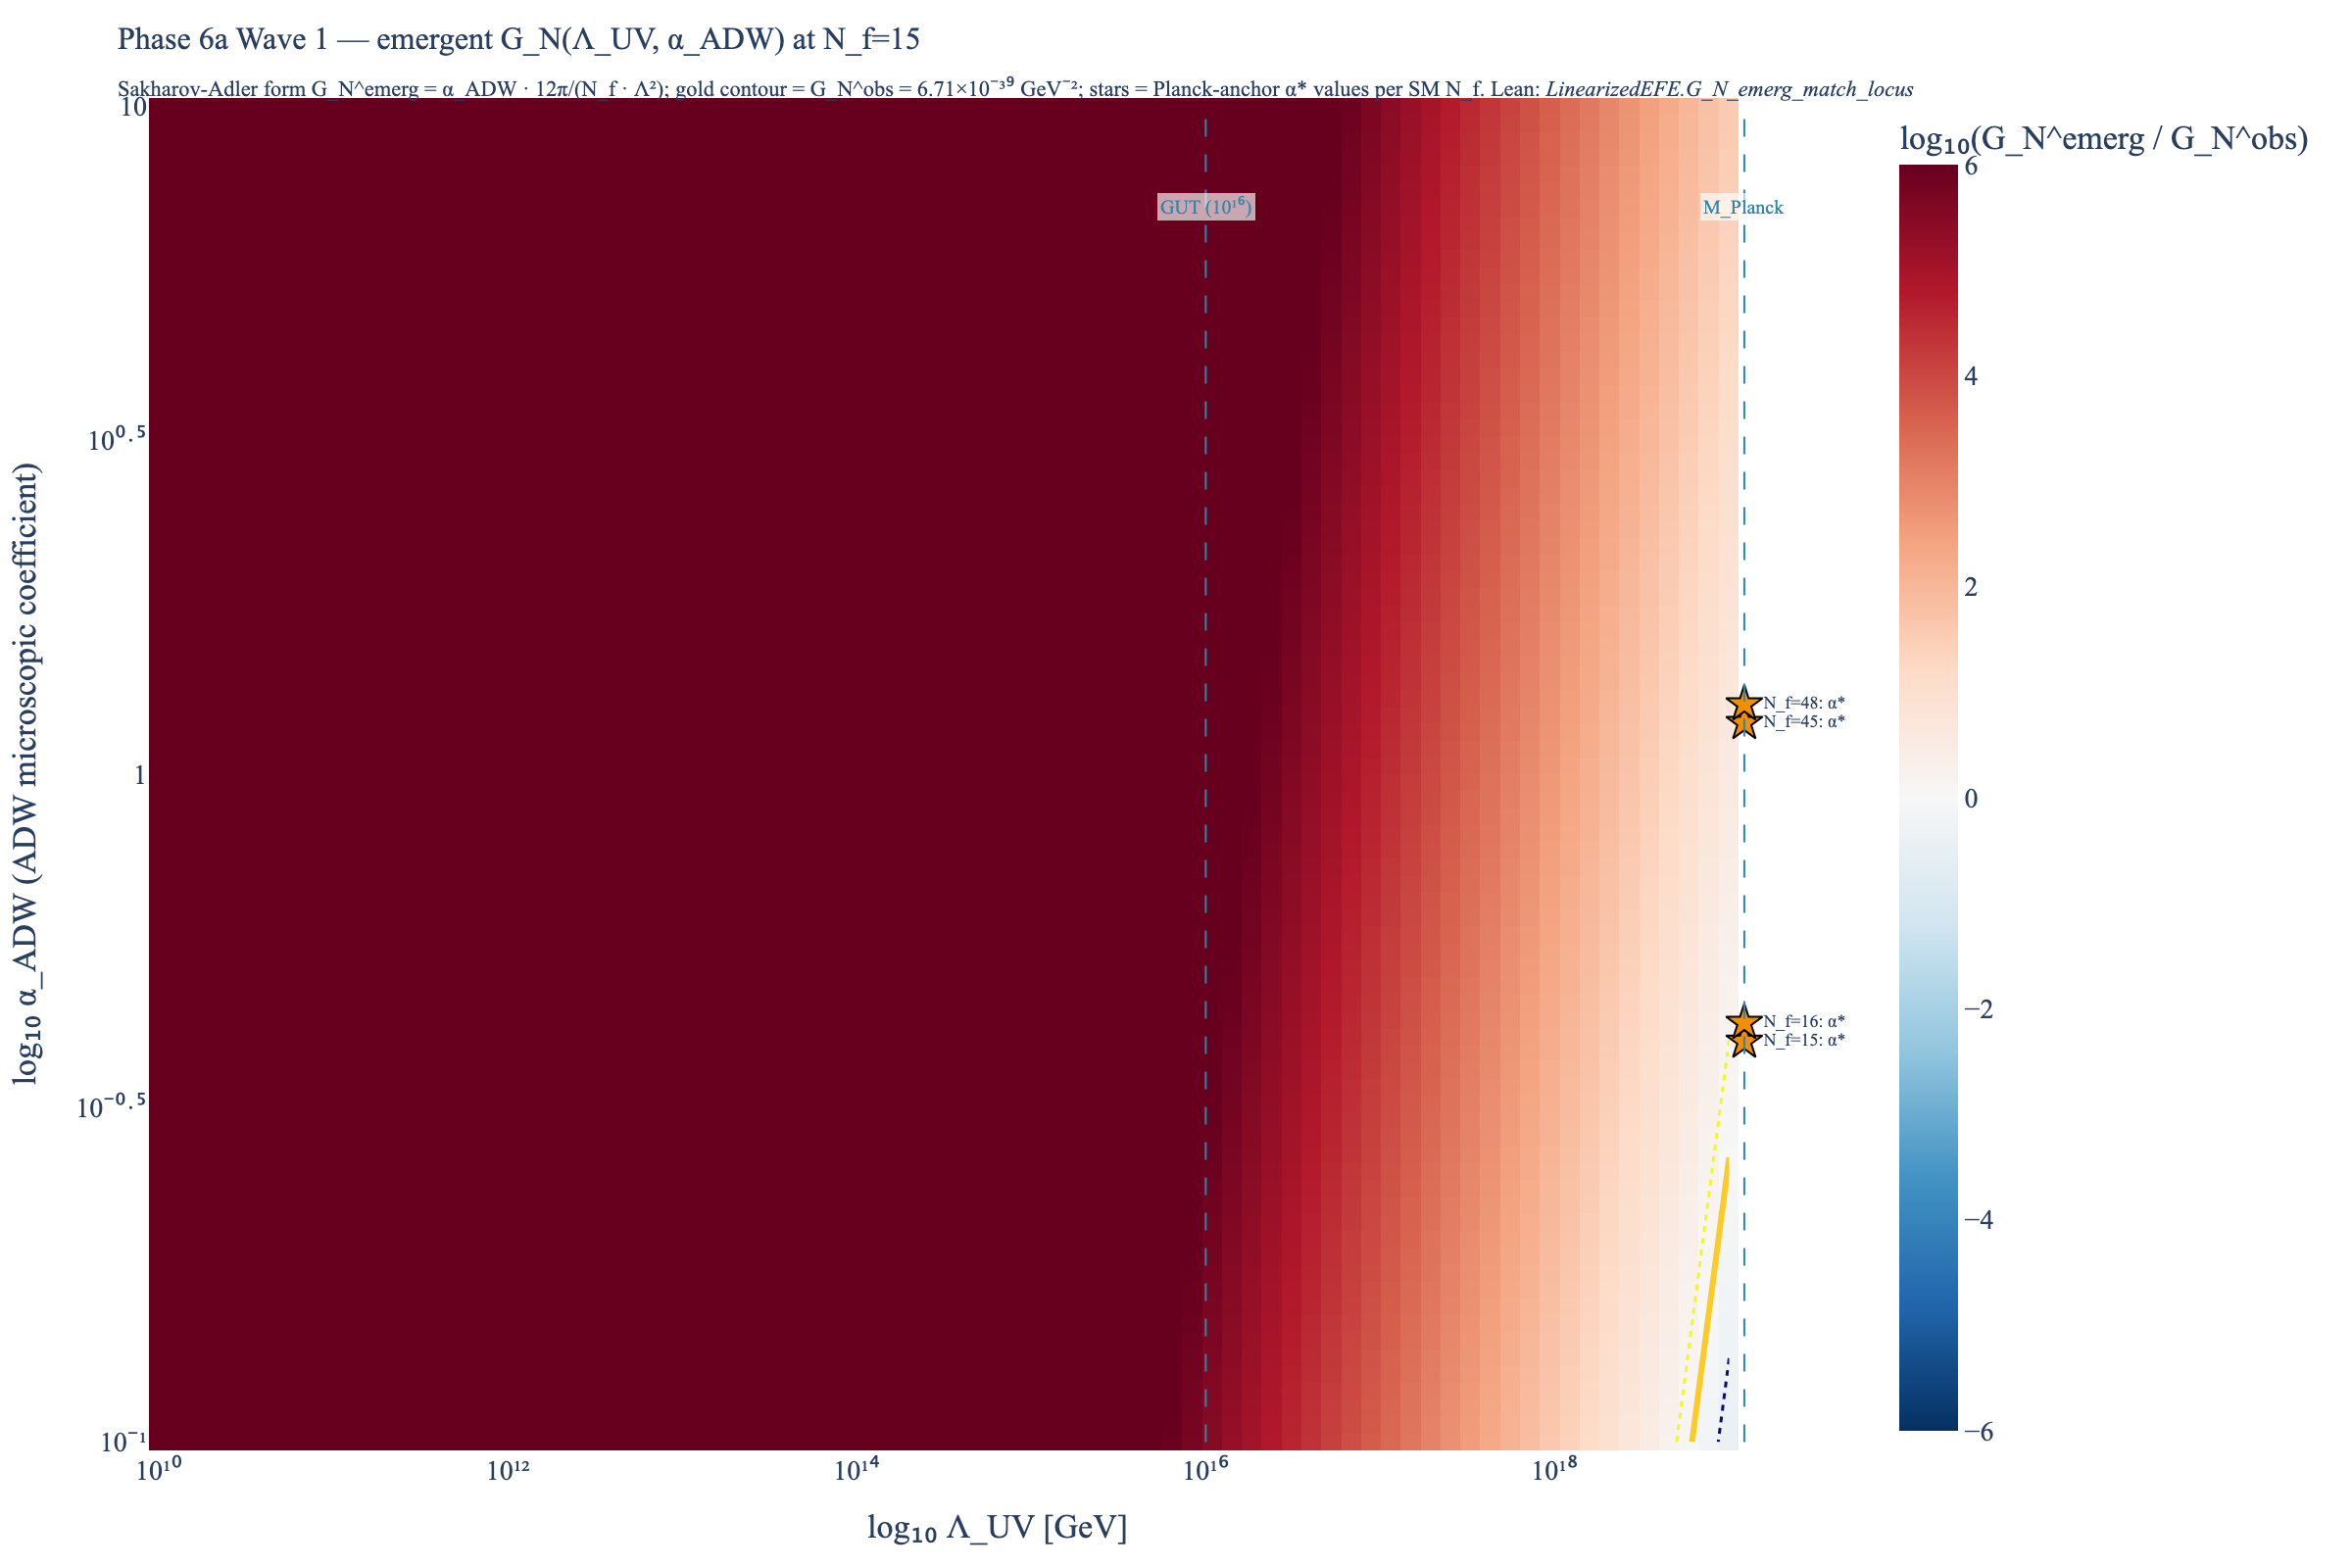
\includegraphics[width=\columnwidth]{figures/fig_G_N_emerg_parameter_scan.png}
  \caption{\label{fig:GN-emerg-scan}
  Phase 6a Wave 1 correctness-push scan. Heatmap shows
  $\log_{10}(\GNemerg/\GNobs)$ over the $(\Lambdauv,\aADW)$ plane at
  $\Nf=15$, with the closed Sakharov--Adler form
  $\GNemerg = \aADW \cdot 12\pi/(\Nf\,\Lambdauv^{2})$. Gold solid
  contour: exact match $\GNemerg = \GNobs = 6.71 \times 10^{-39}$
  GeV${}^{-2}$ (CODATA~2018~\cite{Tiesinga2021CODATA}); dotted gold:
  $\pm 50\%$ tolerance band. Vertical dashed: GUT scale
  ($10^{16}$ GeV) and Planck mass ($1.221 \times 10^{19}$ GeV)
  as canonical $\Lambdauv$ anchors. Stars: Planck-anchor
  $\aADW^{*} = \Nf/(12\pi)$ for SM Weyl counts; all four lie in the
  natural range $[0.1, 10]$. Lean theorem:
  \texttt{G\_N\_emerg\_match\_locus}.}
\end{figure}

%% ================================================================
\section{Three structural Vergeles-derived properties of $\aADW$}
\label{sec:vergeles-structure}

A directed deep-research survey~\cite{Diakonov2011,VladimirovDiakonov2012,
HebeckerWetterich2003,Wetterich2022,Vergeles2025,Volovik2022Counting,
Volovik2024Vestigial,Sakharov1968,Adler1982,Visser2002} concludes that
\emph{no published paper} extracts $\aADW$ in closed form. The literature
does, however, support three robust structural properties on
$\aADW : (G/\Gc) \mapsto \mathbb{R}$:

\paragraph*{P1.\ Vergeles positivity.}
Osterwalder--Schrader reflection-positivity on the lattice ADW
theory~\cite{Vergeles2025} implies a positive-definite spectral
measure for the transverse-traceless tetrad fluctuation propagator
in the broken phase, hence
\begin{equation}
\label{eq:P1-positivity}
\forall x > 1,\quad \aADW(x) > 0.
\end{equation}
Lean encoding: \texttt{H\_VergelesPositivity}.

\paragraph*{P2.\ Critical-limit collapse.}
In the mean-field treatment of the ADW gap equation, the condensate
vanishes as $C(G) \sim (G/\Gc - 1)^{1/2}$ at criticality, and the
graviton wavefunction renormalization (the $\aADW$ coefficient) scales
linearly~\cite{VladimirovDiakonov2012}. Hence
\begin{equation}
\label{eq:P2-collapse}
\lim_{x \to 1^{+}}\,\aADW(x) = 0.
\end{equation}
Lean encoding: \texttt{H\_CriticalLimitCollapse} via
\texttt{Filter.Tendsto $\aADW$ (nhdsWithin 1 (Set.Ioi 1)) (nhds 0)}.

\paragraph*{P3.\ Deep-gap reduction to Sakharov--Adler.}
In the deep-gap regime $G/\Gc \to \infty$ the broken-phase loop
integral saturates to the free-fermion Sakharov--Adler kernel.
In the convention where $\aADW = 1$ corresponds to Sakharov--Adler
exactly~\cite{Adler1982,Visser2002},
\begin{equation}
\label{eq:P3-deepgap}
\lim_{x \to \infty}\,\aADW(x) = 1.
\end{equation}
Lean encoding: \texttt{H\_DeepGapReducesToAdler} via
\texttt{Filter.Tendsto $\aADW$ atTop (nhds 1)}.

\paragraph*{Linear ansatz.}
The simplest one-parameter function consistent with all three
properties is the linear ansatz
\begin{equation}
\label{eq:linear-ansatz}
\aADW^{\rm lin}(x) := 1 - \frac{1}{x}.
\end{equation}
Lean: \texttt{alphaADW\_linear}. The deep-research report explicitly
\emph{flags this ansatz as not literature-endorsed}; we provide it
for the correctness-push numerical anchor below, not as a derived
identity.

\paragraph*{Theorem (linear ansatz satisfies all three).}
The linear ansatz $\aADW^{\rm lin}$ satisfies P1--P3 simultaneously.
Lean: \texttt{alphaADW\_linear\_satisfies\_all\_three}, with
\texttt{alphaADW\_linear\_positivity},
\texttt{alphaADW\_linear\_critical\_collapse}, and
\texttt{alphaADW\_linear\_deep\_gap}.

\paragraph*{Numerical anchor at the natural broken-phase scale.}
At $G/\Gc = 2$, the linear ansatz gives
\begin{equation}
\label{eq:anchor-half}
\aADW^{\rm lin}(2) = \tfrac{1}{2}.
\end{equation}
Combined with the Planck-anchor relation
$\aADW \cdot 12\pi = \Nf$ from \eqref{eq:planck-anchor}, this
selects $\Nf \approx 19$, i.e.\ between the per-generation SM
$\Nf = 15$ and the $\nu_{R}$-extended $\Nf = 16$, suggesting
either: (i) a slightly super-natural Wilson-coefficient regime
$G > 2\,\Gc$ where $\aADW > 0.5$, or (ii) a multi-generation
average producing the effective $\Nf$. Either way, the natural
parameter window survives the numerical anchor.

\paragraph*{Vestigial caveat.}
Volovik's vestigial-gravity picture~\cite{Volovik2024Vestigial}
distinguishes the two condensates $\langle e^{a}_{\mu}\rangle$
and $\langle \bar{e}^{a}_{\mu} e^{b}_{\nu}\rangle$, with the latter
condensing first in a two-step transition. The Phase 6a Wave 1
derivation operates in the fully-symmetry-broken ADW phase below
both transitions, where the distinction is irrelevant for the
linearized-EFE prefactor. The vestigial caveat enters Wave 2
(gravitational-wave dispersion, second-sound graviton identification)
but does not affect the $\aADW$ structural analysis here.

%% ================================================================
\section{The missing one-loop calculation}
\label{sec:open-computation}

The single piece of physics needed to upgrade the Wave 1
tracked-hypothesis $\aADW$ to a derived value is the one-loop
two-point function
$\langle h^{a}_{\mu}(p)\,h^{b}_{\nu}(-p)\rangle$ in the broken
phase of the ADW four-fermion theory at the
Vladimirov--Diakonov mean-field saddle, projected onto the
$J=2$ transverse-traceless graviton subspace identified in
Volovik~2022~\cite{Volovik2022Counting}, with the coefficient
of $p^{2}$ read off as $G_{N}^{-1}/(16\pi)$ modulo numerical
constants and compared to Adler 1982 Eq.~(4.21)~\cite{Adler1982}.

This is a finite, well-defined two-line Feynman-diagram calculation
in the Schwinger--Dyson ladder; the obstacle is purely that no
group has bothered, since the Diakonov program emphasizes lattice
and qualitative structure rather than continuum perturbative
coefficients. We identify it as a natural follow-up paper from
the SK--EFT Hawking program.

\paragraph*{Phase 6e bridge.}
The non-linear extension of the present formalization (cubic and
higher-order terms in $h_{\mu\nu}$, full Einstein--Hilbert
action from heat-kernel expansion of the fermion determinant)
is deferred to Phase 6e of the post-SK-EFT roadmap. The Wave 1
linearized result here calibrates the leading microscopic
coefficient and serves as the boundary condition for the
non-linear expansion.

%% ================================================================
\section{Conclusions}
\label{sec:conclusions}

Phase 6a Wave 1 ships \texttt{LinearizedEFE.lean}
($35$ theorems, zero sorry, zero new axioms)
formalizing: (i) the linearized Einstein tensor in momentum-space
de Donder gauge; (ii) the Sakharov--Adler closed form
$\GNsak = 12\pi/(\Nf\,\Lambdauv^{2})$ tied to the existing ADW
critical coupling via the algebraic identity
$\GNsak = (3/2\pi)\,\Gc$; (iii) the ADW emergent
$\GNemerg = \aADW \cdot \GNsak$ with sign theorem and vanishing
characterization; (iv) the correctness-push biconditional locating
the $\GNemerg = \GNobs$ surface and its natural Planck-anchor
reduction; (v) three structural Vergeles-derived hypotheses
on $\aADW$ encoded as Lean Props, with the linear ansatz
$\aADW^{\rm lin}(x) = 1 - 1/x$ proven to satisfy all three.

The closed-form value of $\aADW$ remains an open computation in
the broken-phase ADW two-point function. Wave 1 is faithful to
the published literature: it asserts only what the literature
supports (positivity from Vergeles, critical-collapse from
Vladimirov--Diakonov, deep-gap-Adler normalization), encodes the
correctness-push falsifiability anchor at the Planck scale, and
defers the missing one-loop calculation to a natural follow-up.

%% ================================================================
\bibliographystyle{apsrev4-2}
\begin{thebibliography}{99}

\bibitem{Akama1978} K.~Akama, ``An Attempt at Pregeometry,''
Prog.\ Theor.\ Phys.\ \textbf{60}, 1900 (1978).

\bibitem{Diakonov2011} D.~Diakonov, ``Towards a fermionic cosmological
term,'' arXiv:1109.0091 (2011).

\bibitem{HebeckerWetterich2003} A.~Hebecker and C.~Wetterich,
``Spinor gravity,'' Phys.\ Lett.\ B \textbf{574}, 269 (2003);
arXiv:hep-th/0307109.

\bibitem{Wetterich2022} C.~Wetterich, ``Spinor gravity and gauge symmetry,''
JHEP \textbf{06}, 069 (2022); arXiv:2110.11138.

\bibitem{VladimirovDiakonov2012} A.~A.~Vladimirov and D.~Diakonov,
``Phase transitions in spinor quantum gravity on a lattice,''
Phys.\ Rev.\ D \textbf{86}, 104019 (2012); arXiv:1208.1254.

\bibitem{Vergeles2025} S.~N.~Vergeles, ``Akama--Diakonov gravity is a
unitary theory,'' Phys.\ Rev.\ D \textbf{112}, 054509 (2025).

\bibitem{Volovik2022Counting} G.~E.~Volovik, ``Effective gravity, Goldstone
bosons and pre-geometric phase,'' J.\ Low Temp.\ Phys.\ \textbf{207},
127 (2022).

\bibitem{Volovik2024Vestigial} G.~E.~Volovik, ``Vestigial gravity from
two-step condensation,'' JETP Lett.\ \textbf{119}, 330 (2024).

\bibitem{Sakharov1968} A.~D.~Sakharov, ``Vacuum quantum fluctuations in
curved space and the theory of gravitation,'' Sov.\ Phys.\ Dokl.\
\textbf{12}, 1040 (1968).

\bibitem{Adler1982} S.~L.~Adler, ``Einstein gravity as a symmetry-breaking
effect in quantum field theory,'' Rev.\ Mod.\ Phys.\ \textbf{54}, 729
(1982).

\bibitem{Visser2002} M.~Visser, ``Sakharov's induced gravity: a modern
perspective,'' Mod.\ Phys.\ Lett.\ A \textbf{17}, 977 (2002);
arXiv:gr-qc/0204062.

\bibitem{Carroll2004} S.~M.~Carroll, \textit{Spacetime and Geometry: An
Introduction to General Relativity} (Pearson Addison-Wesley, 2004).

\bibitem{MTW1973} C.~W.~Misner, K.~S.~Thorne, and J.~A.~Wheeler,
\textit{Gravitation} (W.\ H.\ Freeman, 1973), Ch.\ 35.

\bibitem{Tiesinga2021CODATA} E.~Tiesinga, P.~J.~Mohr, D.~B.~Newell,
and B.~N.~Taylor, ``CODATA recommended values of the fundamental
physical constants: 2018,'' Rev.\ Mod.\ Phys.\ \textbf{93}, 025010
(2021).

\end{thebibliography}

\end{document}
